\documentclass[11pt]{article}
\usepackage[margin=1in]{geometry}
\usepackage[T1]{fontenc}
\usepackage{lmodern}
\usepackage{booktabs}
\usepackage{graphicx}
\usepackage{enumitem}
\usepackage[hidelinks]{hyperref}
\setlist{nosep,leftmargin=1.4em}
\setlength{\parskip}{0.5em}
\setlength{\parindent}{0pt}

\begin{document}

\begin{center}
{\large\bfseries Good Data or Leaked Data?}\\[2pt]
Do Aggregate Privacy Checks Hide Risk to Outlier Records in Synthetic Tabular Data?\\[4pt]
Megha Chaudhari and Austin Qi\\
Course Research Project --- Progress Report
\end{center}

\section*{Response to Proposal Feedback}

The proposal feedback asked for a novel research question rather than a literature review alone. We have narrowed the project to one question that the papers we reviewed do not answer directly, and that we can test with our own experiment:

\begin{quote}
\emph{When a synthetic dataset passes the aggregate privacy check that generator papers commonly report, are outlier records in the training data still exposed at a much higher rate than typical records?}
\end{quote}

Generator papers such as TabDDPM~[3] summarize privacy with a single dataset-level number based on the distance to the closest record (DCR). Stadler et al.~[6] show with targeted attacks that outliers are the records most at risk. No paper we reviewed checks whether the commonly reported aggregate check would reveal that risk. If it does not, a dataset can look safe on paper while its most identifiable people are exposed. The literature review is still part of the project, but it now serves this question: it explains which checks are reported and why they might miss record-level risk.

We test two hypotheses:
\begin{itemize}
\item \textbf{H1.} For a given generator, a simple membership inference attack succeeds more often on outlier records than on typical records.
\item \textbf{H2.} The aggregate DCR check does not reveal this gap: generators can look close to the ideal value while outliers remain more exposed.
\end{itemize}

\section*{Progress on the Literature Review}

We have organized the evaluation measures in our six papers into the four groups from the proposal. Table~\ref{tab:lit} records which groups each paper reports.

\begin{table}[h]
\centering\small
\begin{tabular}{@{}lcccc@{}}
\toprule
Paper & Statistical similarity & Predictive utility & Privacy-risk check & Formal guarantee \\
\midrule
SDV~[1] & yes & yes (human study) & -- & -- \\
CTGAN~[2] & yes (likelihood) & yes & -- & -- \\
TabDDPM~[3] & yes & yes & yes (DCR) & -- \\
RCGAN~[4] & yes (MMD) & yes (TSTR) & yes (memorization) & yes (DP training) \\
Herurkar et al.~[5] & yes (new metrics) & yes (TSTR/TRTS) & -- & -- \\
Stadler et al.~[6] & -- & yes & yes (attacks) & yes (DP models) \\
\bottomrule
\end{tabular}
\caption{Evaluation groups reported by each paper. ``--'' means not tested, not unsafe.}
\label{tab:lit}
\end{table}

Two observations motivate our question. First, the three generator papers that define the field's benchmarks (SDV, CTGAN, Herurkar et al.) report no privacy-risk check at all. Second, where a check is reported (TabDDPM), it is a single dataset-level number. Only the dedicated privacy paper~[6] looks at individual records, and it uses attacks too costly to be routine in generator papers. Our experiment asks whether the cheap aggregate check is enough.

\section*{Experimental Setup}

We use UCI Adult (45,222 complete rows). For each of three random seeds we split it into a training set (5,000 rows) used to fit the generators, a holdout set (5,000 rows) never seen by them, a test set (10,000 rows) for utility, and a reference set (the remaining rows) used only to define outliers. Each generator produces 5,000 synthetic rows. We compare the Gaussian copula~[1], CTGAN~[2] and TVAE~[2] (300 epochs, \texttt{sdv} library), a SMOTE-style interpolation baseline in the spirit of the TabDDPM comparison~[3], and a ``copy'' reference that resamples training rows directly.

\begin{itemize}
\item \textbf{Utility:} train a gradient-boosting classifier on synthetic data, test on real test data (TSTR), and report F1 for the \texttt{>50K} class.
\item \textbf{Aggregate privacy check:} for each synthetic record, find its closest real record and ask whether it lies in the training set or the holdout set. The share closer to training is the \emph{DCR share}; 0.5 means no sign of copying.
\item \textbf{Record-level risk:} a simple membership inference attack scores each real record by its distance to the closest synthetic record. We report the fraction of training members identified at a 1\% false-positive rate (TPR), separately for typical records and outliers.
\item \textbf{Outliers:} the 10\% of training and holdout records with the largest mean distance to their 10 nearest neighbors in the reference set.
\end{itemize}

Distances use standardized numeric features and one-hot categorical features, with scaling fit on the training data only.

\section*{Preliminary Results}

\begin{table}[h]
\centering\small
\begin{tabular}{@{}lcccc@{}}
\toprule
& TSTR F1 & DCR share & \multicolumn{2}{c}{Members identified at 1\% FPR} \\
\cmidrule(l){4-5}
Generator & & (0.5 = ideal) & Typical & Outliers \\
\midrule
Real data (reference) & 0.685 & -- & -- & -- \\
Copy (reference) & 0.668 & 1.000 & 0.635 & 0.629 \\
Interpolation (SMOTE-style) & 0.663 & 0.929 & 0.185 & 0.436 \\
CTGAN & 0.599 & 0.506 & 0.011 & 0.009 \\
TVAE & 0.586 & 0.520 & 0.010 & 0.013 \\
Gaussian copula & 0.083 & 0.517 & 0.010 & 0.017 \\
\bottomrule
\end{tabular}
\caption{Mean over three seeds. Random guessing identifies 1\% of members at 1\% FPR.}
\label{tab:results}
\end{table}

\begin{figure}[h]
\centering
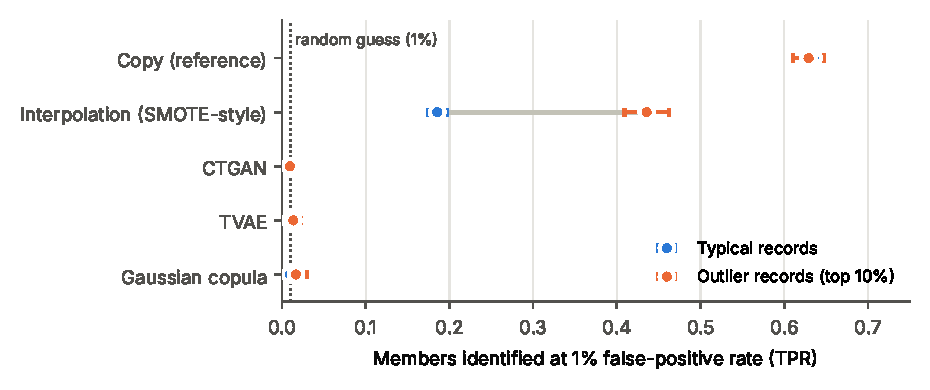
\includegraphics[width=0.85\linewidth]{../results/fig_outlier_risk.pdf}
\caption{Members identified by the attack at a 1\% false-positive rate, typical vs.\ outlier records (mean $\pm$ 1 s.d.\ over three seeds).}
\label{fig:outlier}
\end{figure}

\textbf{H1 holds for interpolation, not for the deep generators.} The SMOTE-style baseline exposes outliers at more than twice the rate of typical records (43.6\% vs.\ 18.5\%, Figure~\ref{fig:outlier}), consistent across all three seeds. Interpolating between a rare record and its nearest neighbor produces points that sit close to that rare record and to few others. CTGAN and TVAE show no measurable leakage with our attack, for outliers or typical records, while keeping most of the real-data utility (F1 0.60 and 0.59 vs.\ 0.69).

\textbf{In this setting the aggregate check is not misleading.} The interpolation baseline that leaks also fails the DCR check clearly (0.93), and the generators that pass it (0.51--0.52) show no leakage. So the natural experiment alone cannot answer H2: no generator here leaks only its outliers.

\textbf{A controlled test supports H2.} To test H2 directly, we start from TVAE output and replace a small number of synthetic rows with near-copies of randomly chosen outlier training records (numeric features jittered by 5\% of a standard deviation, so none is an exact duplicate). This simulates a generator that memorizes only its rarest records. Figure~\ref{fig:planted} shows the result:

\begin{itemize}
\item With 50 planted rows (1\% of the synthetic data), the attack identifies 11.0\% of outlier members, up from 1.3\% with none planted. The DCR share moves only from 0.520 to 0.524, and the exact-duplicate check finds nothing.
\item Even with 250 planted rows, about half of all outlier members (50.8\%) are identified, yet the DCR share (0.545) stays inside the range we observed for the unaltered generators (0.46--0.56).
\item The attack's overall success rate barely moves either (1.0\% to 1.4\%). An average over all records hides the risk as well as the DCR check does.
\end{itemize}

\begin{figure}[h]
\centering
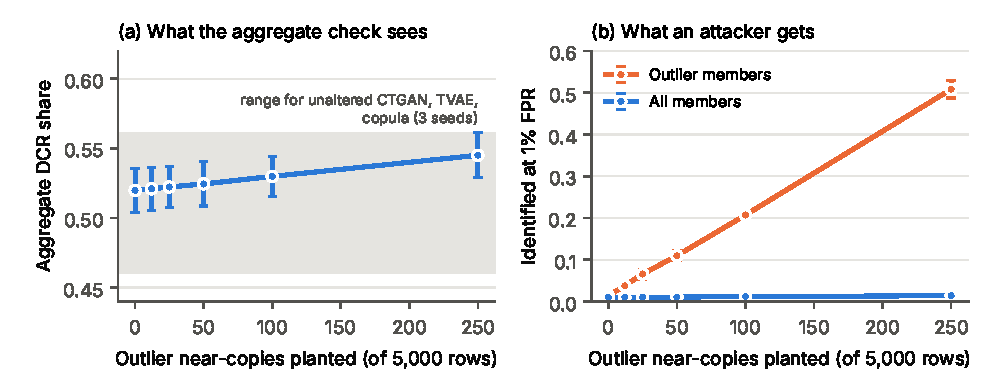
\includegraphics[width=0.95\linewidth]{../results/fig_planted.pdf}
\caption{Planting near-copies of outlier training records into TVAE output (mean $\pm$ 1 s.d.\ over three seeds). (a) The aggregate DCR share stays within the range seen for unaltered generators (gray band). (b) The share of outlier members identified rises roughly linearly, while the overall rate stays near 1\%.}
\label{fig:planted}
\end{figure}

\textbf{Takeaway so far.} A dataset can pass the dataset-level check that generator papers report while exposing a large share of its outliers. The check is only informative when leakage is widespread, as with interpolation. This suggests that privacy evaluations should report attack success on outliers (or another high-risk subgroup) separately, not only an average.

\section*{Remaining Work and Timeline}

\begin{itemize}
\item \textbf{Week 4 (current):} Done: data pipeline, five generators, utility and privacy measures, the planted-leakage test, three random seeds. Next: check that the outlier definition is not driving the result by repeating with a second definition (isolation forest) and a 5\% cut-off.
\item \textbf{Week 5:} Add one stronger attack that uses all synthetic neighbors rather than the single closest record, and a second dataset if time allows. Write the full report.
\item \textbf{Week 6:} Write the checklist (now including a record-level check for outliers), revise, and finalize the notebook.
\end{itemize}

\section*{Challenges and Changes}

\begin{itemize}
\item The Gaussian copula produced poor utility on Adult (Table~\ref{tab:results}), so it is mainly a low-utility, low-leakage reference point. We will report this rather than tune it to look better.
\item Our attack and DCR both depend on how features are encoded and scaled. We fix the encoding on real training data only and document it in the code; results with other encodings may differ.
\item One dataset and three seeds limit how far the results generalize. The planted test shows that the aggregate check \emph{can} miss concentrated leakage. It does not show that real generators leak this way; CTGAN and TVAE did not in our runs. We will present it in those terms.
\item Our attack is deliberately simple. Stronger attacks~[6] might find leakage in CTGAN or TVAE that ours does not, so ``no measurable leakage'' means ``none found by this attack''.
\end{itemize}

Code and results are in our course repository under \texttt{synthetic\_privacy\_project/}.

\section*{References}
{\small
\begin{enumerate}[label={[\arabic*]},leftmargin=2.2em]
\item N. Patki et al. The Synthetic Data Vault. IEEE DSAA, 2016.
\item L. Xu et al. Modeling Tabular Data using Conditional GAN. NeurIPS, 2019.
\item A. Kotelnikov et al. TabDDPM: Modelling Tabular Data with Diffusion Models. ICML, 2023.
\item C. Esteban et al. Real-valued (Medical) Time Series Generation with Recurrent Conditional GANs. arXiv:1706.02633, 2017.
\item D. Herurkar et al. Evaluating Generative Models for Tabular Data: Novel Metrics and Benchmarking. arXiv:2504.20900, 2025.
\item T. Stadler et al. Synthetic Data -- Anonymisation Groundhog Day. USENIX Security, 2022.
\end{enumerate}}

\end{document}
